% Number 100
% CAPM AMM
% Car speeds up, slows down: rel. easy, pairs with 90
% MIT Physics for Teachers LON-CAPA

% Watermark
\AddToShipoutPicture*{\BackgroundPic}

\addtocounter {ProbNum} {1}

%\begin{floatingfigure}[r]{.3\textwidth}
%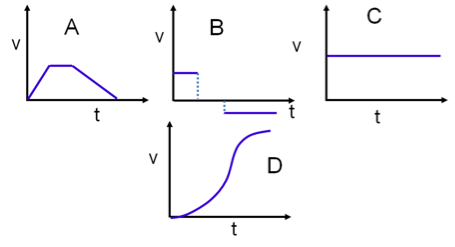
\includegraphics[scale=.4]{/Users/jgates/desktop/latex/pics/vgraph1.png}
%\end{floatingfigure}
 
{\bf \Large{\arabic{ProbNum}}} A car starting from rest speeds up to ${30~\frac{m}{s}}$ with constant acceleration in 15 seconds. Then, it travels at ${30~\frac{m}{s}}$ for 10 seconds. Finally, it brakes to a stop in 30 seconds with constant acceleration. 

 \bigskip

\indent How far does it travel in the 55 second time period?  
 

\vfill

\newpage
